%% ----------------------------------------------------------------
%% Thesis.tex -- MAIN FILE (the one that you compile with LaTeX)
%% ---------------------------------------------------------------- 

% Set up the document
\documentclass[a4paper, 11pt, oneside]{Thesis}  % Use the "Thesis" style, based on the ECS Thesis style by Steve Gunn
\graphicspath{Figures/}  % Location of the graphics files (set up for graphics to be in PDF format)

% Include any extra LaTeX packages required
\usepackage[square, numbers, comma, sort&compress]{natbib}  % Use the "Natbib" style for the references in the Bibliography
\usepackage{verbatim}  % Needed for the "comment" environment to make LaTeX comments
\usepackage{vector}  % Allows "\bvec{}" and "\buvec{}" for "blackboard" style bold vectors in maths
\usepackage[export]{adjustbox}
\hypersetup{urlcolor=blue, colorlinks=true}  % Colours hyperlinks in blue, but this can be distracting if there are many links.

%% ----------------------------------------------------------------
\begin{document}
\frontmatter      % Begin Roman style (i, ii, iii, iv...) page numbering

% Set up the Title Page
\begin{titlepage}
    \begin{center}
        
\includegraphics[width=0.4\textwidth]{Figures/FRA-UAS-Logo.jpg}
        \\
        \vspace*{1cm}
        \title{}
        \LARGE{Masters Thesis Report}\\
        \vspace{2cm}
        \Huge
        \textbf{Automating Flight insurance}\\
        \LARGE{A thesis presented for the degree of\\
        M. Sc. High Integrity Systems}
        
        \vspace{0.5cm}
        \LARGE
        
        
        \vspace{1.5cm}
        
        \textbf{Vineet Chawla}\\
        \small{Matriculation Number: 1118276}
        
        \vspace{2.8cm}
        
        {\LARGE 
		Principal Guide: Prof. Dr. Andreas Orth \\
		Additional Guide: Prof. Dr. Eicke Godehardt \\
		\begin{center}
			Frankfurt University of Applied Sciences \\		
			Fachbereich 2: Informatik \& Ingenieurwissenschaften
		\end{center}
	    }

        	
        
    \end{center}
\end{titlepage}

%% ----------------------------------------------------------------

\setstretch{1.3}  % It is better to have smaller font and larger line spacing than the other way round

% Define the page headers using the FancyHdr package and set up for one-sided printing
\fancyhead{}  % Clears all page headers and footers
\rhead{\thepage}  % Sets the right side header to show the page number
\lhead{}  % Clears the left side page header

\pagestyle{fancy}  % Finally, use the "fancy" page style to implement the FancyHdr headers

%% ----------------------------------------------------------------
% Declaration Page required for the Thesis, your institution may give you a different text to place here
\Declaration{

\addtocontents{toc}{\vspace{1em}}  % Add a gap in the Contents, for aesthetics

I, VINEET CHAWLA, declare that this thesis titled, `Automation Flight Delay Insurance' and the work presented in it are my own. I confirm that:

\begin{itemize} 
\item[\tiny{$\blacksquare$}] This work was done wholly or mainly while in candidature for a Masters degree at this University.
 
\item[\tiny{$\blacksquare$}] Where any part of this thesis has previously been submitted for a degree or any other qualification at this University or any other institution, this has been clearly stated.
 
\item[\tiny{$\blacksquare$}] Where I have consulted the published work of others, this is always clearly attributed.
 
\item[\tiny{$\blacksquare$}] Where I have quoted from the work of others, the source is always given. With the exception of such quotations, this thesis is entirely my own work.
 
\item[\tiny{$\blacksquare$}] I have acknowledged all main sources of help.
 
\item[\tiny{$\blacksquare$}] Where the thesis is based on work done by myself jointly with others, I have made clear exactly what was done by others and what I have contributed myself.
\\
\end{itemize}
 
 
Signed:\\
\rule[1em]{25em}{0.5pt}  % This prints a line for the signature
 
Date:\\
\rule[1em]{25em}{0.5pt}  % This prints a line to write the date
}
\clearpage  % Declaration ended, now start a new page

%% ----------------------------------------------------------------
% The "Funny Quote Page"
\pagestyle{empty}  % No headers or footers for the following pages

\null\vfill
% Now comes the "Funny Quote", written in italics
\textit{``This thesis made me angry''}

\begin{flushright}
Vineet Chawla
\end{flushright}

\vfill\vfill\vfill\vfill\vfill\vfill\null
\clearpage  % Funny Quote page ended, start a new page
%% ----------------------------------------------------------------

% The Abstract Page
\abstract{

The blockchain, decentralised digital ledger, has the potential to disrupt many traditional business models. Insurance industry is one of them. The insurance process is currently based on business practices that haven't changed in decades and as a result, provide the users with less than optimal experience including abnormally long time for claim reimbursement. This paper provides a new direction for flight delay insurance, completely automating insurance process by embracing modern technologies. Fundamentally, we will be automating the underwriter's task of deciding insurance premiums and paybacks using machine learning and provide a legal agreement using blockchain,  essentially automating the whole step of claim management. The user will in turn be provided with higher transparency and less bureaucracy.

}

\clearpage  % Abstract ended, start a new page
%% ----------------------------------------------------------------

\setstretch{1.3}  % Reset the line-spacing to 1.3 for body text (if it has changed)

% The Acknowledgements page, for thanking everyone
\acknowledgements{
\addtocontents{toc}{\vspace{1em}}  % Add a gap in the Contents, for aesthetics

Not completed yet\ldots

}
\clearpage  % End of the Acknowledgements
%% ----------------------------------------------------------------

\pagestyle{fancy}  %The page style headers have been "empty" all this time, now use the "fancy" headers as defined before to bring them back


%% ----------------------------------------------------------------
\lhead{\emph{Contents}}  % Set the left side page header to "Contents"
\tableofcontents  % Write out the Table of Contents

%% ----------------------------------------------------------------
\lhead{\emph{List of Figures}}  % Set the left side page header to "List if Figures"
\listoffigures  % Write out the List of Figures

%% ----------------------------------------------------------------
\lhead{\emph{List of Tables}}  % Set the left side page header to "List of Tables"
\listoftables  % Write out the List of Tables

%% ----------------------------------------------------------------
% End of the pre-able, contents and lists of things
% Begin the Dedication page

\setstretch{1.3}  % Return the line spacing back to 1.3

\pagestyle{empty}  % Page style needs to be empty for this page
\dedicatory{For/Dedicated to/To my\ldots}

\addtocontents{toc}{\vspace{2em}}  % Add a gap in the Contents, for aesthetics


%% ----------------------------------------------------------------
\mainmatter	  % Begin normal, numeric (1,2,3...) page numbering
\pagestyle{fancy}  % Return the page headers back to the "fancy" style
\lhead{\emph{Automating Flight Insurance}}  % Set the left side page

% Include the chapters of the thesis, as separate files

\chapter{Introduction}

Currently the insurance industry is beset with redundant and poorly optimised business processes. In this paper, the focus will be on the airline insurance or specifically, airline delay insurance. The aim will be to optimise the whole insurance process so that the user doesn't have to interact with the insurance portal. Instead of keeping the customer in the dark about the insurance payout and making them apply for the claim, we will try to be completely  transparent with the user. This will be  achieved using these two strategies
\begin{itemize}
    \item We will show the customer payouts if the flight is delayed before the user buys the insurance. This insurance rates will be calculated on the basis of probability of flight getting delayed.
    \item The customer will be assured that the insurance has been created using Blockchain. We will anchor the customer data to Bitcoin blockchain for providing a timestamp of the insurance created. This would not require any third party service for verification.
\end{itemize}

\section{Existing Work}
Even though there have been many commerce services providing commerce applications using Blockchain, there is no particular website that provides a full fledged flight delay insurance capability. A similar project was created on Ethereum smart contract called Etherisc. But using that needed an Ethereum client running on the user's machine and transactions only happened using Ether, severely limiting the functionality and reach of the platform.
On 13\textsuperscript{th} Sept though insurance conglomerate launched a new website called \url{fizzy.axa} that provides the exact functionality as we intend to provide for this project. It calculates the insurance rates and displays them to the user before the user books the insurance. The claim process is automatically triggered with the help of smart contracts on Ethereum blockchain. The only difference seems to be that they pay the user only when the flight is delayed more than 2 hours.

\section{Problem Statement}
Our problem statement can be defined as creating a platform such that the complete process of booking flight insurance is transparent and easy for the user. Once the user selects the flight and the date, the user will be shown the insurance rates before booking the insurance. The claims process will also be completely removed. The user will be automatically notified once the flight has landed and payment will trigger if the flight was delayed.

\section{Objective and Limitations}
The objective of the project is automating the process plain and simple. But the project does not aim to create a full fledged insurance purchasing option yet. Smart contracts are still in infancy and have not gained full legal standing yet. The regulatory hurdles currently for Blockchain to be accepted as accepted platform for auditing by regulatory bodies are immense.
Our prediction also only takes into account flights landing in Germany and only last six months flight.
\\As this is a prototype application, the actual handling of money doesn't take place. The transfer of money is simulated and is defaulted of 10€, unless stated otherwise. 

\section{How the objective will be achieved}
The first step in calculating the insurance rates would be automating the whole process of insurance underwriters. But in doing so we have to balance risks for the company to make sure we do not lose money. This will be achieved in a very simple way. We will try to predict the probability of flight delays with the outcome classified in 4 different categories. The insurance rates for four categories will be decided on the basis of our prediction results. If we predict the flight is not going to get delayed, we will provide the user with higher payout. If we predict the flight is going to get delayed, we make sure the payout to the user id decreased. This will help us to balance the payout to the users. The exact algorithm to calculate the insurance rates is discussed in the later chapters. 
 % Introduction

\chapter{Blockchain}

Predicting the flight delays to set the insurance rates is half the innovation for this new platform. The other half would be overhauling the current insurance's legal aspects. The platform's aim is to make a digital legal agreement between the insurance platform and the user, which is non-repudiable, irrefutable, time-stamped and can be fully trusted by the customers as well as the regulators. Currently the legal agreements involve Notaries and laborious manual legal work, even for a simple agreement. Using Blockchain, creating such a legal agreement could be automated, resulting in efficiency improvements. Before delving into how blockchain forms part of this product, a short introduction to bitcoin and it's core parts will be focused upon. 

\section{Introduction to Bitcoin}
Blockchain technology was first described in a paper written by Satoshi Nakamoto in his highly influential paper introducing Bitcoin \cite{Nakamoto2008Bitcoin:System}.In the paper, Nakamoto described Bitcoin as a purely peer-to-peer version of electronic cash that would allow online payments to be sent directly from one party to another without going through a financial institution. The core idea of Bitcoin was not new and had been under research for decades, but up until then these ideas were theoretical and had not been successfully implemented \cite{Chaum1983BlindPayments}. To understand how it achieves do such a thing, it is important to understand the basic architecture of Bitcoin. It can essentially be divided in three main components that are mentioned below\cite{Economist2013HowWork}.

\subsection{Blockchain}
A shared public ledger on which the entire Bitcoin network relies. All transactions, once confirmed, are included in the blockchain. Instead of maintaining the balance of each account, Bitcoin wallets calculate their spendable balance via going through previous transactions and calculating the bitcoins  still owned by the spender. The integrity and the chronological order of the blockchain transactions are enforced with strong cryptography to prevent unauthorised manipulation. 

\subsection{Private Keys}
A transaction is a transfer of value between Bitcoin wallets that gets included in the block chain. Each bitcoin wallet keeps a secret  private key or seed, which is used to sign each transaction, providing a mathematical proof that the transaction has come from the owner of the wallet. The signature also prevents the transactions from being altered by anybody once they are issued. All transactions committed by users are broadcast publicly and usually begin to be confirmed by the Bitcoin network within 10 minutes, through a process called mining.

\subsection{Mining}
Mining is a distributed consensus system used by many cryptocurrencies to confirm valid, waiting transactions and including them in the blockchain. It enforces a chronological order of transactions in the block chain, protects the neutrality of the network, and allows different users/systems to agree on the state of the system. To be confirmed, transactions must be packed in a block, validated by very strict cryptographic rules that are always verified by the network. The hashes added to each block, prevent previous blocks from being modified because doing so would invalidate the current block's hash. Mining also creates the equivalent of a competitive lottery that prevents any individual from easily adding new blocks consecutively in the block chain. This way, no individual can control what is included in the block chain or replace parts of the block chain to roll back their own spending transactions.

\section{More details on Blockchain}
As discussed above, Blockchain is what is now known as a public distributed ledger, designed in the first place to solve the double spending problem, that is, to establish consensus in a decentralised network over who owns what and what has already been spent\cite{Nakamoto2008Bitcoin:System}. 

A distributed ledger is essentially an asset database that can be shared across a network of multiple sites, geographies or institutions. All participants within the blockchain network can have their own identical copy of the digital ledger. Any changes to the ledger are reflected in all copies in minutes, or in some cases, seconds. The assets can be financial, legal, physical or electronic. The security and accuracy of the assets stored in the ledger are maintained cryptographically through the use of private keys and signatures to control who can do what within the shared ledger. Entries can also be updated by one, some or all of the participants, according to rules agreed by the network.\cite{Walport2015DistributedChain}
So how does Blockchain help in keeping records of Bitcoin transactions. Blockchain enables Bitcoin transactions to be aggregated in ‘blocks’ and these are added to a ‘chain’ of existing blocks using a cryptographic signature. The Bitcoin ledger is constructed in a distributed and ‘permission-less’ fashion, so that anyone can add a block of transactions if they can solve a new cryptographic puzzle to add each new block, also known as mining as explained above. The incentive for solving the puzzle, or mining in Bitcoin terms, is that each miner gets a reward for each time the block they mined is added to the blockchain.\cite{Nakamoto2008Bitcoin:System}

\section{Benefits of Blockchain}
What we have when abstracting a blockchain network to a certain level is a distributed, self-authenticating, time-stamped store of data\cite{MonaxBlockchains}. Indeed, the core design of a blockchain node is an elegant way of overcoming many challenges faced by legacy distributed systems.

\subsection{Resilient Data Management System}
Blockchain clients allow for the development of distributed systems which do not rely on what traditional databases with ‘master-slave’ architecture rely upon. Blockchain networks utilise the idea of peer nodes and consensus models to resolve the current state of the data. It means it relies on a consortium of computers which validate the data through the defined consensus model, in effect increasing fault tolerance and resiliency of the system. On the other hand, breaking the data-driven transactions into blocks allows the consensus of the database to be negotiated between the miners in a reasonable manner rather than on a per-transaction basis.

\subsection{Increased Verifiability}
Blockchain networks also allow for transactional certainty due to its basic design and architecture. Traditional databases save the current state of the data, and generally, have additional entries covering previous transactions within the data store. In addition, traditional databases also maintain logs of the history of the interactions.
\\Blockchain networks are designed differently in that the previous transactions of a node are used to formulate the current state of the node and corresponding data. The general blockchain design not only requires that the transactional history of the data store is captured, but that it is cryptographically certain once there is sufficient consensus within the network. The use of cryptographic authentication of time-stamped blocks of transactions allows the entire network the benefit of certainty of the entire transactional history.

\section{Potential of Blockchain}
Blockchain technology came to the limelight as it was the basis of cryptocurrencies such as Bitcoin and Ethereum, but its capabilities extend far beyond that, enabling existing technology applications to be vastly improved. The new platform described in this paper would not be possible without utilising this technology. Blockchain is expected to revolutionise both industry and commerce, and drive economic change on a global scale due to ability to provide immutable and transparent transactions.  As the transaction on Blockchain can be public or private, it could empower people in developing countries with recognised identity, asset ownership, and financial inclusion; and it could avert a repeat of the 2008 financial crisis, support effective health care programs, improve supply chains and, perhaps, clean up unethical behaviour in high-value businesses such as diamond trading.\cite{Underwood2016BlockchainBitcoin}

\subsection{Impact on Financial Industry}
The area where Blockchain can have immediate and everlasting effect in the current financial services is the back-office handling of transactions. When a financial institution sells a syndicated loan or derivative, the recording of the transaction is time consuming and involves burdensome back-office processes. These processes rely on negotiated contracts with the numerous associated lawyers and contact between the parties to finish the transaction. On average, it can take 20 days to settle a syndicated loan trade. These back-end activities are also costly to the financial institutions. This is in contrast to the front-end systems at financial institutions, where millions are spent to achieve a nanosecond of competitive advantage. In addition, financial institutions, due to regulatory requirements, are dealing with greater requirements for reporting, transparency, and dissemination of data. They need a technological breakthrough to help solve these problems. Blockchain can be the breakthrough that can streamline these financial transactions. There are estimates that Blockchain could save financial institutions at least \$20 billion annually in settlement, regulatory, and cross-border payment costs.\cite{Fanning2016BlockchainServices}

\begin{itemize}
    \item Fintech startup R3, backed by over 40 of biggest global banks and financial institutions, is developing a standardised architecture for private ledgers that could significantly cut the cost and time of settling transactions\cite{Brown2016Corda:Introduction}. It is called Corda and currently in beta phase. More will be discussed about Corda in latter sections.
    \item The Linux Foundation’s Hyperledger project is an industry initiative created with IBM's collaboration that is evolving open source technology and building the foundation of a standardised, production grade digital ledger\cite{IBM2015LinuxTechnology}.
    \item Deloitte has been working with clients and startups to develop solutions including Smart Identity, which can support banks’ regulatory client onboarding and Know Your Customer (KYC) processes, while individual financial institutions, insurance companies, exchanges, and solutions vendors also have thrown their weight behind blockchain\cite{Chollet2017DeloitteRelease}.
    \item Nasdaq is using its Linq blockchain technology to complete and record private securities transactions, and the Depository Trust \& Clearing Corporation, working with market participants and technology firm Axoni, is managing post-trade events for credit default swaps. Regulators are also interested in the technology, as its transparency and integrity allow market activity to be monitored in real time\cite{Briganti2015NasdaqBlockchain}. 
\end{itemize}


\subsection{Impact on Commerce and Record Keeping}
\begin{itemize}
    \item There is a company called Factom whose sole focus is on securing data. The company is participating in the Honduran land registry project and working on a number of projects in China, including data infrastructure for 80 smart cities, financial technology solutions, and integrating blockchain technology with electronic data notarisation services to enhance integrity in information management. 
    \item Another company called Everledger’s focus is on the identity and legitimacy of objects. Blockchain works well here because its history cannot be changed and it enables trust by consensus. The company’s initial work provides a distributed ledger of diamond ownership and transaction history verification for owners, insurance companies, claimants, and law enforcement agencies. The system assists with prevention of fraud in the supply chain, but also helps consumers decide whether to buy particular diamonds.
\end{itemize}

\section{Smart Contract}
As already discussed, Blockchain provides a base to build a platform that can act as a reliable data store providing transparency, integrity and increased verifiability. Smart contract is a legal agreement that is built on Blockchain itself providing all the benefits of the blockchain and the service of a legal agreement. The smart contracts are automatable by computer, although some parts may require human input and control. The smart contract is enforceable either by legal enforcement of rights and obligations or via tamper-proof execution of computer code.\cite{Clack2016SmartDirections}
In simple words, a smart contract is a digitally enforceable contract without specifying what aspect is being enforced; for smart legal contracts these might be complex rights and obligations, whereas for smart contract code what is being enforced may simply be some predetermined actions of the code.
\\These scripts are compiled into low level operation codes and stored in the blockchain’s data store at a particular address – which is determined when the contracts are deployed to the blockchain. When a transaction is sent to that address the distributed virtual machine on every full node of the blockchain network executes the script’s operation codes using the data which is sent with the transaction. \cite{MonaxContracts}
\\Due to their inherent design Smart contracts are modular, repeatable, autonomous scripts, which can be used to build applications for self, for a community, for a client, for a bounty, or even just for fun. They can be mixed and matched, are easy to iterate, and combined with preset templates for faster creation.
They can be coded to reflect any kind of business or engineering logic which is data-driven: from actions as simple as up-voting a post on a forum, to the more complex such as loan collateralisation and futures contracts, to the highly complex such as repayment prioritisation on a structured note.

\section{Benefits of Smart Contracts}
As blockchain is a secure technology, so smart contracts can be more secure than traditional contract law. Also, they can reduce a number of transaction costs associated with contracting, since the blockchain cuts out any middlemen. However, the fact remains that the quality of the output depends on the quality of the input. Smart contracts are by no means magical constructs that understand user intent and are always flawless. If there is an oversight in the text, the result might be even more dramatic than in a traditional contract, because the rules of the smart contract are recorded in computer code and cannot be freely interpreted according to ‘the intent of the contract’, but only according to literal meaning.

\section{Using Blockchain for flight delay insurance}
Now we will discuss the actual use of Blockchain for the flight delay insurance platform. The original plan for the platform was to use smart contracts for the legal insurance contract between the user and the company. Due to technical difficulties discussed below, the use of smart contract was dropped. In this section, the smart contract platforms evaluated and reason for not using each of the platform is touched upon.

\subsection{Monax}
Monax is a platform that provides developers a free platform to build and run Smart contracts. The platform is based on nodes of Ethereum Virtual machines. There are no limitations on what the platform can do as Turing complete code can be run on Ethereum virtual machines. The smart contracts can be for claims Management or Supply chain management etc. Monax also provides premium SDKs for sectors such as insurance but as they were expensive and only available to a verified developer/company, they were not evaluated for the project. Instead the contract was developed from scratch using their platform with Solidity programming language running on Ethereum virtual machine. 
\subsubsection{Architecture}
For creating a permissioned blockchain on Monax platform, one machine is  required to act as Administrator with full rights and capabilities, and at least three machines are required to act as validator nodes, whose only job will be to validate transactions through consensus. The users that will buy insurance will have a participant account, that has the rights limited to just interact with the blockchain.
\\As Monax is a relatively new company, during the time this evaluation was going on, their product was in an alpha stage. Due to which there were many problems in setup. But as with small companies, it was easy to get in touch with the company's developers and get all  issues pertaining to initial setup fixed. 
\\After setting up with one administrator node, 3 validator nodes and 2 participant nodes, we go through setting up certificates for each machine. Then we create account types and initial tokens. After creating the tokens we give the command to create chains, which will create initial directories for each account created. Once all the directories are created, the mining starts and the genesis block\footnote{Initial block of a cryptocurrency is called a genesis block} is created.
\\Once the smart contract platform is running and mining transactions, a smart contract can be created using solidity and commit transactions between participants.

\subsubsection{Issues faced}
Once the initial setup was over, there were architectural restrictions on what could be done in the platform that made it unsuitable for this platform. 
\begin{itemize}
    \item The participants can't be created on the fly. The initial idea was whenever a user is created, that user should be classified as a participant. This will ensure the smart contract is maintained between the user and the administrator node. But creating a participant means to restart the blockchain initialisation process.
    \item The complete blockchain runs in an Ethereum Virtual machine. There is no way to interact with the actual blockchain. Monax had a node.js library to interact with the blockchain but no official library for Python. As the project is using Python, using a different and new language was not considered due to time constraints.
\end{itemize}

\subsection{Corda}
Already discussed earlier in the paper, Corda is arguably the most famous platform for smart Contracts. It is developed by R3 consortium, which is supported by over 50 of the biggest financial institutions of the world.
\subsubsection{Architecture}
A Corda network is an authenticated peer-to-peer network of nodes, where each node is a JVM run-time environment hosting Corda services and executing applications known as CorDapps.\cite{Hearn2016Corda:Ledger}. This whole network of nodes is in a permissioned network and each node uses point to point communication instead of global broadcast of requests. Instead of every node seeing every transaction between themselves, a node in Corda network can only see a transaction if the node was part of that transaction, but each node still can validate the transaction. This ensures privacy of transactions in a network.
As each node is running a JVM run-time environment, the smart contract, or CorDapp has to be written in a JVM compatible language, like Java or Kotlin.

\subsubsection{Issues faced}
As in the case with Monax, it is not possible to interact with Corda Blockchain directly. But Corda has native support for an Oracle. Oracles are network services that, upon request, provide commands that encapsulate a specific fact (e.g. the exchange rate at time x) and list the oracle as a required signer.\cite{OraclesDocumentation}. So it was planned to create an oracle for getting flight status. The oracle service though can't be created the way REST API service is created. This had to be done with a third-party website such as \url{oraclize.it}. They provided tools necessary to get the data we want as a oracle service. But again, oraclize.it is not free to use and they have to be emailed about the requirements and project on email for getting their service. The whole process was followed to create an oracle service, but it unfortunately didn't bear any fruit.
\\The other reason for dropping the Corda platform was that it's architecture is designed in such a way that suits a limited number of entities which had multiple transactions in between them, as can be seen in the figure \ref{fig:corda_architecture}
\begin{figure}
    \centering
    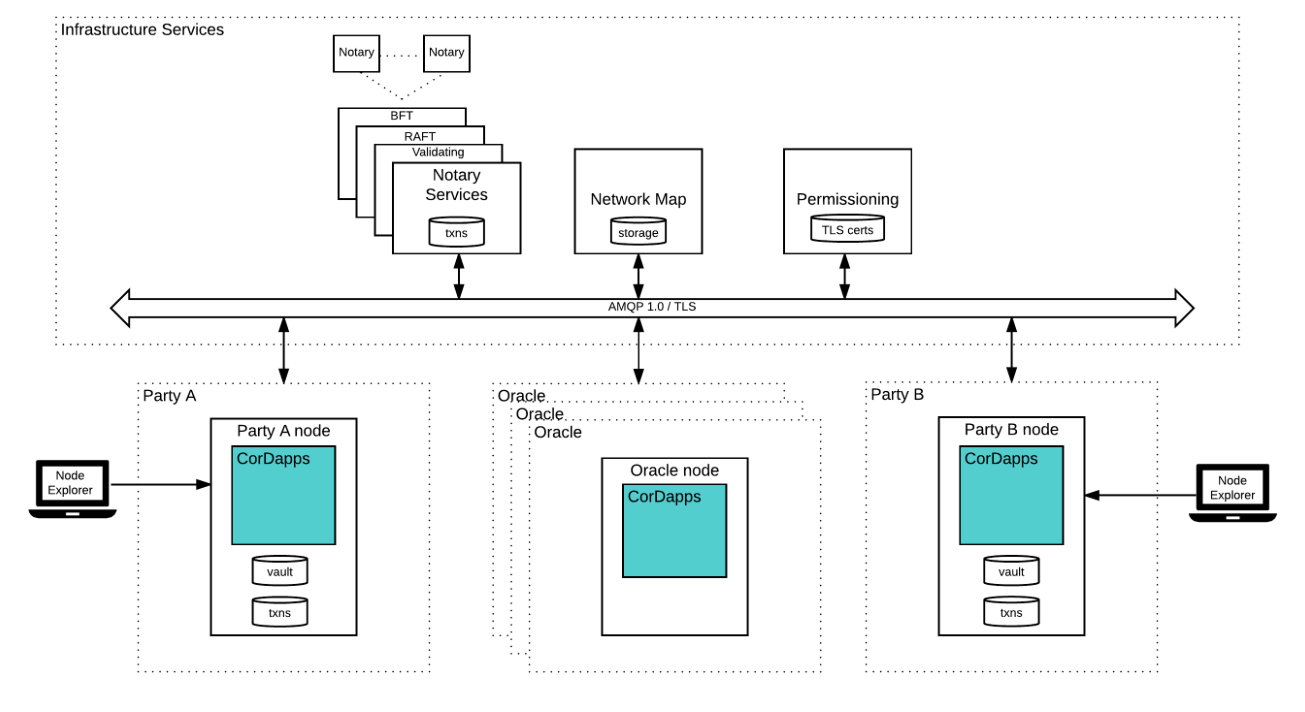
\includegraphics[width=\textwidth]{Figures/corda_architecture.png}
    \caption{Corda's architecture}
    \label{fig:corda_architecture}
\end{figure}.
This was contrary to the project idea for this thesis and consequently, the idea was dropped.


\section{Anchoring data to Blockchain}
Due to time constraints, the whole idea of creating smart contract on a blockchain was dropped and instead the plan for utilising the already existing Bitcoin blockchain was made. This plan was fulfilled by the concept called anchoring of data on Bitcoin blockchain.
\\The use of the Bitcoin blockchain to timestamp and verify data in an immutable public ledger was pioneered by Manuel Aráoz with the creation of Proof of Existence\cite{Araoz2013ProofExistence}. This system, and others like it, notarise data in the blockchain by calculating a hash of the data and publishing it in a Bitcoin transaction. By comparing the hash published in the blockchain with the hash of the same data, it's possible to verify that the data existed at a specific time, providing a mechanism to validate a timestamp.
Anchoring in blockchain simply means adding your data to Bitcoin blockchain to provide irrefutable time-stamps and non-repudiation \cite{Lemieux2017Blockchain:}. There are multiple services that provide anchoring service for valuable data. For this project, Chainpoint was selected as they have a very easy to use (and still free) REST API called Tierion to anchor data to Bitcoin blockchain. Their API provides the anchoring service using anchoring standard they created, Chainpoint.
\\Chainpoint links a hash of the specified data to a blockchain and returns a timestamp proof. A Chainpoint service receives hashes which are aggregated together using a Merkle tree. The root of this tree is anchored in the Bitcoin and Ethereum blockchains. Throughout this process a Chainpoint proof is created and continually upgraded. The final Chainpoint proof defines a path of operations that cryptographically links the specified data to one or more blockchains.\cite{ChainpointStandard}
\\A Chainpoint proof is a JSON-LD document, that contains the information to cryptographically verify a piece of data is anchored to a blockchain. It proves the data existed at time it was anchored. Chainpoint proofs can be verified without reliance on a trusted third party.
\footnote{JSON-LD is a lightweight Linked Data format described here \url{https://json-ld.org/}}
\\Once the data is sent to Tierion through their API, they generate a unique SHA 256 hash of the data. Multiple hashes are assembled into a block, which is simply a list of hashes. Periodically, these blocks are used to generate a Merkle Tree\cite{Merkle1980ProtocolsCryptosystems} , and the Merkle Root is published in the blockchain via a transaction. By collating multiple hashes into a Merkle Tree and publishing the Merkle Root, large volumes of data is anchored in the blockchain using a single transaction. \cite{Wayne2016Chainpoint:Receipts}

\subsection{Blockchain receipts}
Once the data is anchored, the insurance platform should also be able to provide the proof that the data has been hashed to the blockchain network and can be verified via third party too. In the real world, a receipt provides proof of a transaction. In this project's case, a blockchain receipt provides proof that some data existed at a specific time. It contains all the information needed to prove an individual hash was part of the Merkle Tree whose root was published in a transaction in the Blockchain. The data in the blockchain receipt is given in table \ref{table:receipt} and the use of fields to verify data is visually represented in figure \ref{fig:merkle}
\begin{table}[h!]
\centering
\begin{tabular}{||c c||} 
\hline
Name & Description  \\ [0.5ex] 
\hline\hline
@context & the JSON-LD context for the receipt \\ 
\hline
type & receipt type definition specifying hash method and version \\
\hline
targetHash & hash value being anchored to the blockchain \\
\hline
merkleRoot	& merkle tree root value that is anchored to the blockchain \\
\hline
proof	& merkle proof establishing link from the targetHash to the merkleRoot \\
\hline
anchor-type	& anchor type definition specifying anchoring method \\
\hline
anchor-sourceId &	identifier, such as a transaction id, used to locate anchored data \\ [1ex]
 \hline
\end{tabular}
\caption{Different fields in blockchain receipt}
\label{table:receipt}
\end{table}

\begin{figure}[ht]
    \centering
    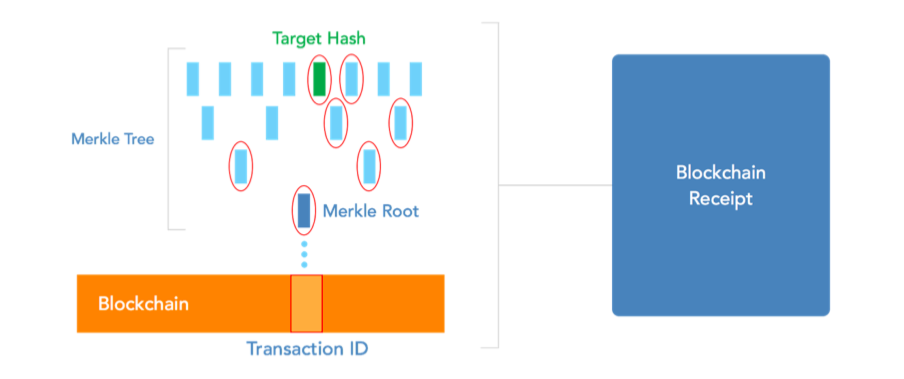
\includegraphics[width=\textwidth]{Figures/Merkle.png}
    \caption{Visual explanation of concept behind blockchain receipt\cite{Wayne2016Chainpoint:Receipts}}
    \label{fig:merkle}
\end{figure}

By tracing a path from the Merkle root to the target hash, a Merkle Proof can be generated that proves any one of the elements is in the Merkle tree, without having to know the entire tree.

\subsection{Integration with project}
The integration of data with Tierion was completed as explained in the following sequence:
\begin{itemize}
    \item Once the user selects and agrees to the shown insurance rates, a JSON string is created with user, flight and insurance data.
    \item The JSON string is sent to Tierion using REST API.
    \item A unique ID of the transaction is received as a response back from Tierion.
    \item Initially the status of the blockchain in unpublished and blockchain receipt is not received. However, within 10 minutes, the status is updated to published and the blockchain receipt is received. ID received earlier is used for updating the status of the transaction and blockchain receipt.
\end{itemize} % Blockchain

\chapter{Flight Data}
To begin with the insurance platform, getting data to predict flight delays is the very first step. For accurate prediction, historical data for each flight landing in Germany will be required. One can easily find many open source datasets of historical flight records, but they are limited to United States flight data. As there is no dataset available that fits the project's needs, a new dataset had to be created from scratch that contains all the flight details of Germany for six months. A large number of websites do provide the status of flights but the ones providing historical flight details are few and expensive. For this reason the requirements were defined for the suitable website in the latter sections and the website was selected on the basis of that criteria. Before creating the historical flight dataset though, there is a need to create another smaller dataset. The list of all flights landing in Germany on any given day.

\section{List of all flights landing in Germany}
Getting the list of every flight landing in Germany on a typical day was not an onerous task. The task was divided into two sub-tasks, first of which was getting the complete list of airports in Germany. A quick glance on Flightradar24 website shows the list of 56 airports handling the chartered and commercial flights\footnote{\url{https://www.flightradar24.com/data/airports/germany}}. Airports which handle only chartered flights were not considered. For each airport, a list was available that had records of all the flights landing in that airport on a given day. Each record for these airport was copied into an Excel file, with the most important flight details like destination, origin, airline and flight ID. On completing the copying, the final list consisted of 3000 flights, flying to or within Germany on a given day, from more than 200 airports worldwide.

\section{Plausible Sources for historical flight data}
The next step was to get the historical data of at least 3 months for each flight in the newly created list. Considering that this was going to be a huge dataset that could not be created/curated manually, the requirements for selecting the flightdata's source were defined beforehand as follows:
\begin{enumerate}
    \item The flight data source should have at least 3 months of historical records of flights, especially the actual departure, actual arrival and flight delay.
    \item The flight data source should preferably have a developer friendly API to automate the whole process of retrieving the data.
    \item The API calls limit and subscription costs, if any, for the source should be reasonable.
\end{enumerate}

Based on the above mentioned criteria, the following websites that provide flight records were evaluated.

\subsection{Flightstats}
Flightstats states that it provides the historical data of flights to its registered users. It also provides a REST based API available to its registered users. Registering is not a big issue generally but in case of FlightStats, it is a rather cumbersome ordeal. The user has to give specific domain where the data collected from their website will be used, assure FlightStats there will be no commercial use and give details of what kind of data would be required. On making the request multiple times, my request was rejected. Later a call was made by Flightstats sales team that offered me to provide the complete dataset of historical records of six months of each German flight, as an excel file. The happiness of receiving the complete and clean data was shortlived though as the company asked \EUR{2000} for the dataset, a discounted price for students, which was otherwise double of what was quoted. Hence Flightstats was not considered anymore.

\subsection{Flightaware}
Flightaware on the other hand had an easy registration process. Their developer API is well documented and provides REST API support. Even the developer key is provided free of cost on request. The limitation of the free account is that historical records of only 14 days are provided. A special tier, available for \EUR{20} per month, does provide access to last 5 months of historical flight records\footnote{\url{https://flightaware.com/commercial/premium/}}. But on further research, it was noted that  the historical data was just for display. Their API, FlightXML 3 doesn't provide any particular support for making REST requests for historical data of a flight\footnote{\url{[https://flightaware.com/commercial/flightxml/pricing_class.rvt}}. Hence Flightaware too was not selected.

\subsection{Flightradar24}
Flightradar24 is one of the most famous sites on internet with mobile apps available for iPhone and Android. Flightradar24 does have historical data of 6 months for their Gold tier customers at just \$4 per month. Unfortunately, Flightradar24 provides no API to retrieve that data automatically. Being out of options, this site was selected on the basis of providing maximum amount of data and providing the cheapest premium option.

\section{Getting data}
Not having an API for getting flight history was an obstacle in collecting data. The only option remaining to retrieve the data was scraping it from their webpage. Web Scraping is a technique in which the desired data is extracted from a webpage's HTML output. Having the flight records of last 6 month of flight records as a webpage meant the whole dataset could be created by scraping the data.
\\Even though some websites specifically consider web scraping illegal\cite{Hirschey2014SymbioticScraping}, flightradar24 only rejects web-scraping of data if that data is to be used commercially. The proposed website being a master thesis project, doesn't fit under the commercial category, neither provides anyone actual commercial service. 

\subsection{Web Scraping}
As mentioned earlier, web scraping is basically looking into the source code of a webpage and saving the data desired. Using the previously created list of flights landing in Germany on any given day, a list of URLs was created with the help of this URL template \url{https://www.flightradar24.com/data/flights/<flight_id>/}, where flight\_id was replaced with the Flight ID of each of the flights. 
Once the list of all the web-URLs to be scraped was completed, the actual scraping was started. The language of choice for scraping is Python, as the website was also to be created using Python. The commonly used python library, Scrapy, was used for scraping. Each of the URLs in the list prepared earlier was passed as argument to Scrapy HTTP request function and the desired data variables from  the HTTP response received were saved.
 

\section{Data Variables}
All the data  retrieved from scraping was saved in a CSV file. The total flight records saved were about 385,000. Once completed, the dataset consisted of the following variables.
\begin{enumerate}
    \item {Departure Airport}
    \\Origin Airport of the flight. This value could be of any airport in the world that has a direct flight to a German airport
    \item {Arrival Airport}
    \\Destination airport of the flight. Always one of the German airports
    \item {Standard Arrival}
    \\The fixed arrival time of a flight time based on the flight schedule, mentioned in the flight plans submitted to the airports
    \item {Actual Arrival}
    \\The actual arrival of the flight, that might be earlier or most probably at or after the standard arrival of the flight
    \item {Standard Departure}
    \\The fixed departure time of a flight time based on the flight schedule, mentioned in the flight plans submitted to the airports.
    \item {Actual Departure}
    \\The actual departure of the flight, that might be earlier or most probably at or after the standard departure of the flight
    \item {Airline}
    \\The company operating the flight.
    \item {Flight ID}
    \\The flight ID is a unique number provided by International Air Transport Organisation to each flight.
    \item {Aircraft}
    \\The type of aircraft for the flight.
    \item {Flight Duration}
    \\Total duration of flight in hours.
\end{enumerate}

\section{Data Cleanup and missing values substitution}
On close inspection of the CSV file with all the stored flight records, it was noted that a lot of columns had some missing values. Hence the next step was to fill in the missing data and correct the incorrect data. One big advantage in cleaning the data was that lots of columns were repetitive in nature. For ex., arrival and destination airports stay same for the flight no matter the date of flight. They were easily fixed. But some of the columns, like flight duration would change everyday. Thus different strategies were created for cleaning missing values for each variable. Microsoft Excel was selected for data cleanup due to its ease of use and data visualisation capabilities.

\subsection{Departure Airport}
Departure Airport stays constant for each Flight ID. In the dataset though, some of the flight IDs had different Departure Airports on few occasions, and few were missing the value. This was rectified for each of the 3000 different flights.

\subsection{Arrival Airport}
The same strategy was applied to Arrival Airport for cleanup as well. But arrival airport had two exceptions as compared to departure airport that had to be considered while cleaning the column.
\begin{enumerate}
    \item Flight diverted
    \\Arrival airport remains constant for each Flight ID except in case the flight is diverted. This was a special case and only happened nine times in the dataset. All these entries were removed from the dataset for the sake of uniformity.
    \item Connecting Flights
    \\There are many indirect flight that connect to German airports. For sake of simplicity, it was decided to keep only flights lading in Germany. For ex, if a flight flew from Delhi to Moscow, and then from Moscow to Frankfurt, only flight that came from Moscow was considered and all details of Delhi-Moscow flight were discarded. 
\end{enumerate} 

\subsection{Standard Arrival}
The Standard Arrival time of a flight does not necessarily stay the same all year long. For ex., it changes on the basis of daylight savings or even as a business decision by an airport or Airline. So
instead of making all values of standard departure same for all historical records of a particular flight, the values for the empty cells were copied from the upper or lower cell in the data belonging to the same flight.

\subsection{Standard Departure}
The same strategy as for Standard Arrival was used for cleaning up Standard Departure too.

\subsection{Actual Arrival}
Arguably the most important variable in the dataset. The actual flight delay will be calculated using this variable. Any row that didn't have this value was removed from the dataset.

\subsection{Actual Departure}
Any values that were missing from actual departure, were assumed to be the same as standard departure.

\subsection{Airline}
Any missing value in the airline column was corrected on the basis of the upper or lower cells in the column. 

\subsection{Flight ID}
This was the basis of the whole web scraping process. Only the flights that had Flight ID were scraped, hence there was no chance of a missing or wrong Flight ID. Still, if there were any repetitions of a Flight ID, the rows were deleted.

\subsection{Aircraft}
For cleaning the missing data in Aircraft, it was assumed that a flight uses same aircraft unless a pattern is noticed where each flight after a certain date uses a different aircraft. Missing values were corrected on the basis of the upper or lower cells in the column.

\subsection{Flight duration}
Another very important variable in the dataset. Any missing value was calculated by subtracting Actual departure from Actual Arrival. All the values were also converted into seconds instead of keeping them in Time format. Any row with flight duration more than 24 hours was deleted.

\section{Adding new variables}
After cleaning the dataset, it was decided to add new variables to the dataset which would hopefully make the predictions better aligned to the project's end goal.

\subsection{Flight delay bins}
The insurance rates provided to the user will be varied based on the flight delay prediction. It was decided that the delays would be calculated based on the following four categories. The goal of the prediction would be to classify the flight delay as one of this class.
\begin{enumerate}
    \item 0 if a flight is less than 15 minutes late
    \item 1 if a flight is 15 or minutes but less than an hour late
    \item 2 if a flight is more than 15 minutes but less than an hour late
    \item 3 if a flight is an hour or more late
\end{enumerate}

\subsection{Weekend}
A simple variable. Using Weekday formula in Excel, a binary variable was created with the value as True if the flight was on weekends and False otherwise.

\subsection{Time Blocks}
Instead of using exact arrival time of the flight, a new variable was created which categorised time to a block of 2 hours duration. For ex., a flight at 8:30 in the morning was classified to block 8 and flight at 15:30 was classified to block 16.

\section{Reducing number of factors}
One problem frequently faced while executing classification algorithms on such a big dataset is the number of categories, or factors, of each variable. The flight records dataset has more than 50 airlines and 80 aircrafts. Algorithms in R like random forest don't accept more than 32 categories. Boosting algorithms like XGBoost on the other hand require indicator columns instead of categorical variables. Converting to indicator columns means that a single column with n categories is converted to n binary columns. Having columns with large number of categories will result in huge number of indicator columns. For these reasons, the categories for some of the columns were reduced.

\subsection{Airline}
There were 67 different airlines in the dataset with Lufthansa being the most popular with 124940 flight records. A large number of airlines though have a comparatively small number of flights. On that basis, it was decided that the airlines with lowest number of flights should be combined in a new airline category called other\_airline.

\begin{figure}[H]
    \centering
    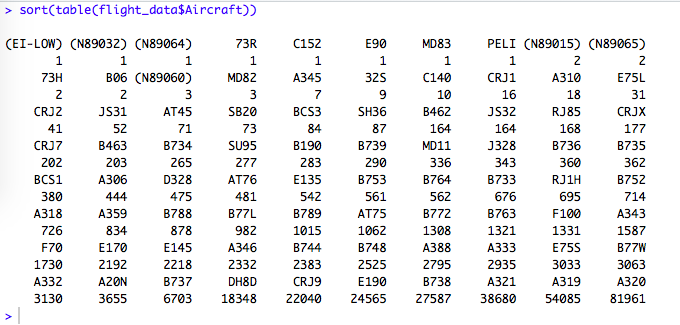
\includegraphics[width=\textwidth]{Figures/Aircraft_orig_levels.png}
    \caption{Reduced categories of Airlines with number of airline}
    \label{fig:airline2}
\end{figure}

\subsection{Aircraft}
There were about 80 different aircrafts in the dataset, with Airbus A320 being the most common choice, having over 81000 flight records. As can be seen in the figure \ref{fig:aircraft1}, there were large number of aircrafts with a insignificant number of flights.

\begin{figure}[H]
    \centering
    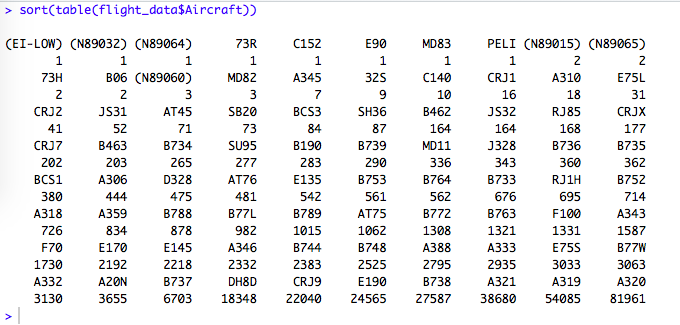
\includegraphics[width=\textwidth]{Figures/Aircraft_orig_levels.png}
    \caption{Original categories of Aircraft with number of flights}
    \label{fig:aircraft1}
\end{figure}

All the aircrafts with the lowest number of flight records were combined to form a new value called other\_aircraft, as seen in figure \ref{fig:aircraft2}.

\begin{figure}[H]
    \centering
    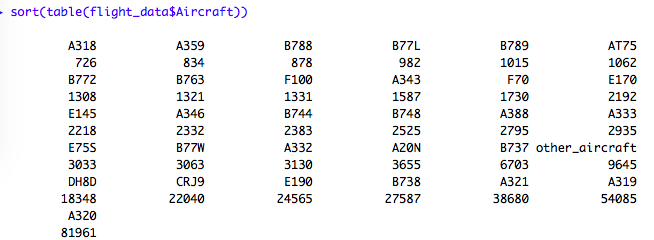
\includegraphics[width=\textwidth]{Figures/Aircraft_reduced_levels.png}
    \caption{Reduced categories of Aircraft with number of flights}
    \label{fig:aircraft2}
\end{figure}

\subsection{Departure Airport}
The departure airport has 287 different departure airports from all over the world. Many of the airports have non-insignificant number of flights so converting a majority of flights to a single category would have been counter-productive. Hence the variable was left as it is 
to. The variable was instead used to create a column with each airport mapped to a country. This is discussed in more detail in the Delay Prediction chapter.

\section{End result - dataset}

After cleaning the data, substituting the missing values, reducing the number of factors and adding new variables to help in prediction, the final summary of the dataset is as seen in figure \ref{fig:summary_flights}:

\begin{figure}[ht]
    \centering
    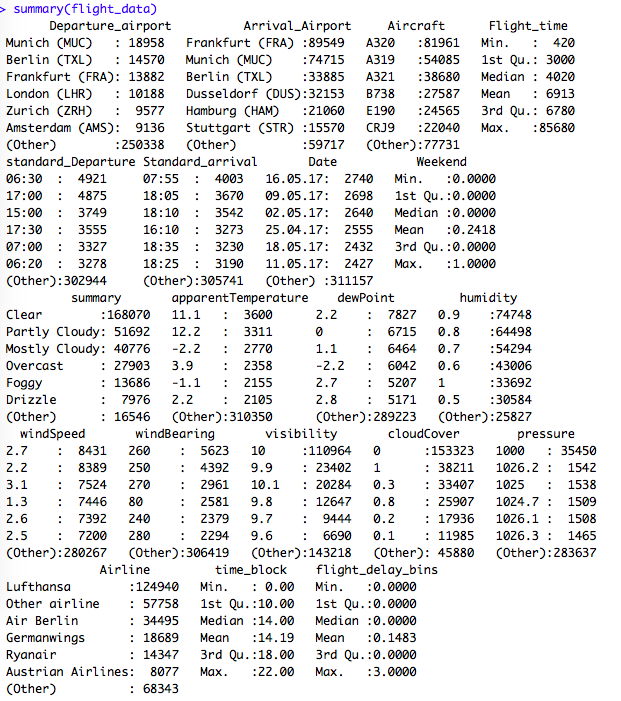
\includegraphics[width=\textwidth]{Figures/summary_flight_data.png}
    \caption{Final summary of our flight dataset}
    \label{fig:summary_flights}
\end{figure} % Flight Data

\chapter{Weather Data}
To further make the training dataset more comprehensive, it was decided to integrate the weather data in with the historical flight details. The plan was to add a multitude of the weather characteristics of the Arrival airport at the time of the arrival of the flight.

\section{Plausible sources for weather data}
Thankfully, collecting historical weather data is much more widespread than collecting historical flight data. As a result, there were many options to choose from, all of which provided a rich developer API.
\\The considerations for choosing weather data provider were based on these two conditions
\begin{enumerate}
    \item Limitations on making API calls
    \item Cost of making API calls
\end{enumerate}
The following three providers were shortlisted and evaluated on the above stated criteria:

\subsection{Apixu}
Although not a famous website, apixu provides historical data of upto a year ago. The subscription of a premium plan of 30 Euros per month is required for the privilege though. It's a reasonable cost but the API has limitations of 300,000 calls per month. For normal use cases this is enough, but for this dataset, it was not enough.

\subsection{openweathermap}
Openweathermap is another famous weather data provider. They have multiple plans for providing historical weather data, but the one that would be suitable for this project would be 950 Euros per month\footnote{\url{http://openweathermap.org/price}}. This is way too expensive for the data so this option was taken out of consideration too.

\subsection{DarkSky API}
Darksky is another weather data provider, lending its data to a famous weather site called \url{Forecast.io}. There is no monthly subscription for this API. Instead the costs are based on the API calls made by the developer. They provide a possibility of 1000 calls every day for free with every subsequent call charged at just \EUR{.00001}. This totalled to only 35 euros for complete data that was required, hence this was a suitable choice. 

\section{Getting data}
Using API from Darksky is easy but the parameters it required were not available in the correct format, or missing altogether from the dataset. 
\begin{enumerate}
    \item Latitude and Longitude
    \\ The latitude and longitude for each airport in Germany was not available anywhere so this information was collected manually using Google maps. In Google maps, once we point to a location, the latitude and longitude of that point are available in its URL. This process was repeated for all the airports in the dataset and then synced to the dataset for each flight.
    \item Time
    \\Even though the time of flight and the date for each record was available, this API required time in UNIX epoch format, number of seconds that have elapsed since 1\textsuperscript{st} January 1970. Using date and actual arrival time of each flight, a new variable was created which had the corresponding epoch format time.
\end{enumerate}

After these new variables were integrated into the dataset, the REST API calls were generated. As with other API calls, the script to get the data was written in python and the data was integrated right into the CSV file containing flight dataset. The following data variables were saved from the requests for each flight.

\begin{enumerate}
    \item Summary
    \\A human-readable text summary of the weather at the time.
    \item Humidity
    \\The relative humidity, between 0 and 1, inclusive
    \item Cloud cover
    \\The percentage of sky occluded by clouds, between 0 and 1, inclusive
    \item Visibility
    \\The average visibility in kilometres, capped at 10 kilometres
    \item Wind Speed
    \\The wind speed in kilometres per hour
    \item Wind Bearing
    \\The direction that the wind is coming from in degrees, with true north at 0° and progressing clockwise. (If windSpeed was zero, then this value was not defined.)
    \item Apparent Temperature
    \\The apparent (or “feels like”) temperature in degrees Celsius.
    \item Dew Point
    \\The percentage of sky occluded by clouds, between 0 and 1, inclusive
    \item Pressure
    \\The sea-level air pressure in millibars.
    \item Precipitation Intensity
    \\The intensity (in inches of liquid water per hour) of precipitation occurring at the given time. This value is conditional on probability (that is, assuming any precipitation occurs at all) for minute data points, and unconditional otherwise.
\end{enumerate}

\section{Missing values cleanup}
As the data was already clean before requesting, the data for each of the flight record was received. The python script used to request the temperature also made sure each value was in sync with the actual flight records.
But there were still many values that were missing in the dataset. The missing variables were less than 100 for all the weather variables. Instead of substituting mean values, to fix this, it was assumed that the weather at same time and location on a day would be very similar to the day before or after. Hence this strategy was used and the missing values were substituted with values above or below the data cell. Rows with outliers were removed from the dataset and a row with multiple 0 values in 3 or more weather variables was removed too. % Weather data

\chapter{Predicting flight delay}
In this chapter, the focus is upon prediction of flight delays using the historical flight dataset created. But before moving on to the actual prediction let's revisit the main aim of the predicting flight delays.
\\The work of underwriters in the insurance industry is to decide the insurance payout rates. It is a complicated process with many terms and conditions, and where consumer interest is not the first priority. The flight delay prediction will help in automating this whole process. Additionally, in a bid to be more transparent to the customer, the payout rates will be shown to the user before buying the insurance so that the user can take a better decision for themselves. The rates will be based on the probability of flights getting delayed. In simple terms, if the model predicts a high probability of delay, the insurance payout will be lower. If the model predicts a low probability of delay, the insurance payout will be higher.
\\Two considerations that should be kept in mind as the reason for predicting the flight delays correctly.
\begin{enumerate}
    \item If the flight is predicted to be delayed, the insurance payouts will be lower for the flight. If a high number of flights are predicted incorrectly as delayed, the consumers are going to see lower payout rates for most of the flights. This will reduce the consumer interest in the platform.
    \item If the flight is predicted to be on-time, the insurance payouts will be higher for the flight. If a large number of flights are predicted incorrectly as on-time, the consumers are going to see high payout rates for most of the flights. This will be a loss-making proposition for the platform so should be avoided.
\end{enumerate}

\section{Exploratory Data Analysis}
It's a good idea to look at the dataset before starting the prediction. Some of the relations between variables are discovered through exploratory data analysis and it will help in setting the direction for data analysis.
\\The first relationship to focus on is the average delays at the airports as well as airlines. For the sake of clarity, only top eight airlines are chosen. 

\begin{figure*}[h]
    \centering
    \begin{subfigure}[h]{0.5\textwidth}
        \centering
        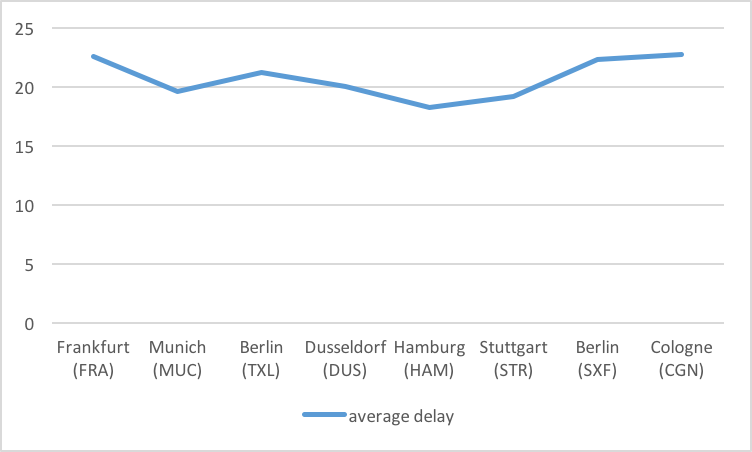
\includegraphics[height=1.7in]{Figures/airport_delay.png}
        \caption{Average delay at top destination airports}
    \end{subfigure}%
    ~ 
    \begin{subfigure}[h]{0.5\textwidth}
        \centering
        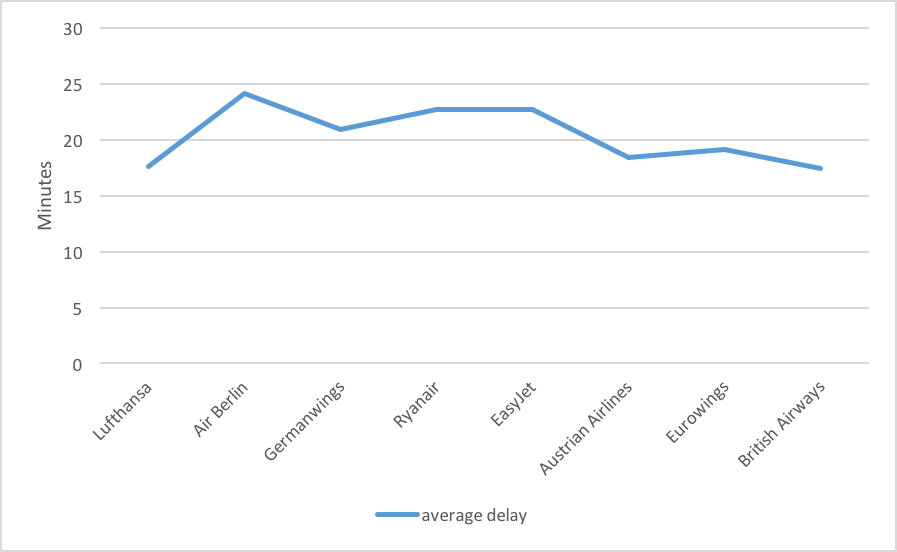
\includegraphics[height=1.7in]{Figures/airline_delay.png}
        \caption{Average delay of top airlines}
    \end{subfigure}
    \caption{Average delay in minutes}
\end{figure*}

Next important consideration is the ratio of delayed flights to flights on time. In the figures, the ratio can be seen for top 8 airlines as well as airports

\begin{figure*}[h]
    \centering
    \begin{subfigure}[h]{0.5\textwidth}
        \centering
        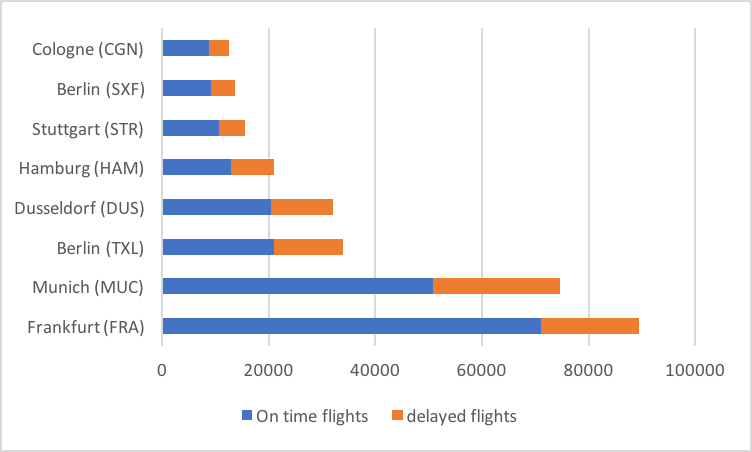
\includegraphics[height=1.7in]{Figures/airport_delay_ratio.png}
        \caption{Delayed flights vs On-time flights for top airlines}
    \end{subfigure}%
    ~ 
    \begin{subfigure}[h]{0.5\textwidth}
        \centering
        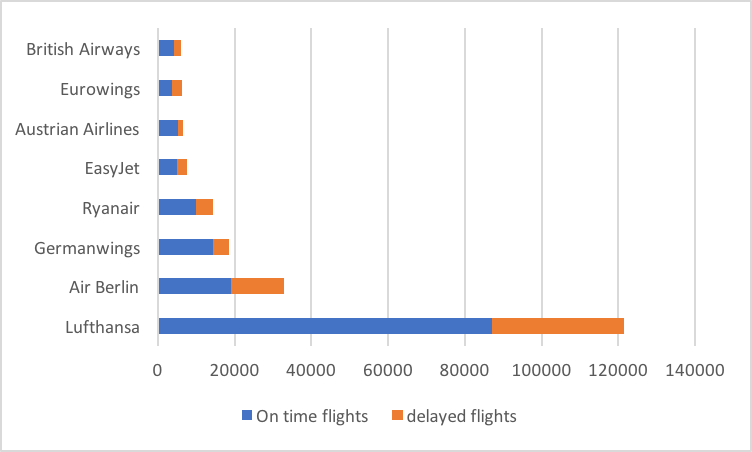
\includegraphics[height=1.7in]{Figures/airline_delay_ratio.png}
        \caption{Delayed flights vs On-time flights for top airlines}
    \end{subfigure}
    \caption{Delayed flights vs On-time flights}
\end{figure*}


\section{Prediction}
The prediction techniques can be classified into two categories, classification and regression. As already mentioned, the target variable for the desired model would contain four prediction classes. The classification algorithms directly classify predicted delay to these four classes. The regression technique on the other hand predicts flight delay in minutes. The flight delay classes will be calculated using the delayed minutes.

\subsection{Implementation}
All the algorithms were first tested using RStudio in R language. For testing different prediction algorithms, the dataset was divided into a training and test dataset. The training set was 75\% of the whole dataset and the test set, on which the prediction was performed, was the remaining 25\%. The algorithm finalised was implemented in python for real time prediction of flight delays on the web platform.

\subsection{Confusion matrix}
The accuracy of any prediction model can be measured by prediction error. But in this case, there is a substantial number of flights that are not delayed ($>$80\%). If the model predicts all flights as not delayed, the accuracy will be $>$80\%, an excellent prediction normally, but what is deceiving in this particular case. Due to this predicament, each model was evaluated using confusion matrix. The confusion matrix is often used to describe the performance of classification model. It is a table showing the actual values in rows and how they were predicted by the model, mentioned in columns. 
%\begin{figure}[H]
%    \centering
%    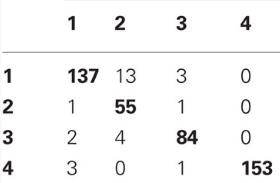
\includegraphics[]{Figures/confusion_matrix_ex.png}
%    \caption{Example of a confusion matrix}
%    \label{fig:confusion_matrix_ex}
%\end{figure}

\begin{wrapfigure}{R}{0.5\textwidth} 
\vspace{-20pt}
  \begin{center}
    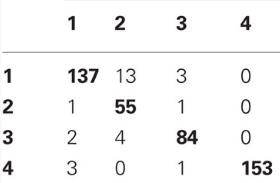
\includegraphics[width=0.4\textwidth]{Figures/confusion_matrix_ex.png}
    \caption{Example of a confusion matrix}
    \label{fig:confusion_matrix_ex}
  \end{center}
  \vspace{-20pt}
  \vspace{1pt}
\end{wrapfigure} 

As seen in figure \ref{fig:confusion_matrix_ex}, the rows are the actual values and the columns are the predicted values. Taking the first row as context, the actual value is 1. 137 is the number of values predicted correctly as 1. 13 is the number of values where the correct prediction was 1 but the model predicted 2, and so on. In essence, the diagonal values of a confusion matrix are the correct predictions, and the model's aim will be to increase the diagonal values.

\section{Prediction using Classification}
In statistics, classification is the problem of identifying to which of a set of categories belongs to which observation. An example would be assigning a given object into "sphere" or "non-sphere" classes or assigning a piece of code as "virus", "suspicious" or "not virus" based on certain characteristics of the operations the code performs.
\\An algorithm that implements classification is known as a classifier. These classifiers are further divided into binary classifiers, those that classify to only two classes, and multiclass algorithms, the ones which will be used for this dataset.

\subsection{Random Forest}
Random forest is an ensemble learning method for classification (and regression) that operates by constructing a multitude of decision trees at training time and outputting the class that is the mode(the value that appears most often) of the classes output by individual trees.\cite{TinKamHoRandomForests}
It is an improvement of decision trees algorithm, which had a habit of overfitting to their training set\cite{Winham2013APerformance}.
\\There are multiple packages that implement random forest in R, the most famous being \textit{randomForest}. But instead the package used for this model is called \textit{ranger}. The latter is used because it exploits the full potential of a multiclass architecture and is much faster than the original implementation. Starting with the predictions, with default parameters, and running with a count of 100 trees, the confusion matrix calculated is as shown in table \ref{table:cm_rf_100}.

\begin{table}[H]
\centering
\begin{tabular}{l | a | b | a | b | a}
\hline
\rowcolor{LightCyan}
\mc{1}{Actual Delay class}  & \mc{1}{Class 0} & \mc{1}{Class 1} & \mc{1}{Class 2} & \mc{1}{Class 3} & \mc{1}{Grand Total} \\
\hline
Class 0 & 71066 & 565 & 35 & 11 & 71677 \\
Class 1 & 6920 & 1280 & 41 & 4 & 8245\\ 
Class 2 & 962 & 168 & 168 & 1 & 1299\\
Class 3 & 322 & 25 & 16 & 58 & 421\\ \hline
Grand Total & 79270 & 2038 & 260 & 74 & 81642
\end{tabular}
\caption{Classification using Random Forest, 100 trees}
\label{table:cm_rf_100}
\end{table}

As this is the first confusion matrix calculated, it's prudent that it should be discussed in detail. The ensuing ones won't be discussed in such detail.
\\With a test set of about 81000 flights among which 71677 flights were on time, the model correctly predicts no delay(class 0) for 71066 flights. Among those incorrectly predicted as not delayed, 565 were classified as class 1(delay less than an hour), 35 were classified as class 2(delayed more than an hour) and 11 were classified as class 3 (delayed more than 2 hours). 
\\Now let's go through the row of class 2. These belong to flights that were delayed for more than an hour. The correct flights predicted with class 2 were 168, whereas 962 flights were declared as not-delayed. This behaviour can be seen for all delay classes. The prediction models overwhelmingly classify flights as not delayed even though they were delayed. The next step is to optimise the model to improve the prediction of flights delayed.

Optimising the random forest parameters is possible using the \textit{caret} package. The algorithm was tuned using the code as follows

\begin{lstlisting}[language=R, breaklines=true]
tr <- trainControl(method = "cv", number = 5)
train( train\$flight_delay_bins ~ .,data=train,method="rf",trControl= tr)
\end{lstlisting}

The output of the optimisation process using cross validation among multiple random forest models was that the variable \textit{mtry} should be set to 3. It is the number of variables available for splitting at each tree node. Further explanation for the variable is out of the scope of this Thesis. For each of the following models, \textit{mtry} was kept to 3. The next way to optimise the algorithm was using different number of trees for the algorithm. The result is as follows.


\begin{table}[H]
\centering
\begin{tabular}{l | a | b | a | b | a}
\hline
\rowcolor{LightCyan}
\mc{1}{Actual Delay class}  & \mc{1}{Class 0} & \mc{1}{Class 1} & \mc{1}{Class 2} & \mc{1}{Class 3} & \mc{1}{Grand Total} \\
\hline
Class 0 & 71018 & 608 & 38 & 13 & 71677 \\
Class 1 & 6902 & 1294 & 43 & 6 & 8245\\ 
Class 2 & 976 & 163 & 160 & 0 & 1299\\
Class 3 & 323 & 22 & 17 & 58 & 59\\ \hline
Grand Total & 79219 & 2087 & 258 & 78 & 81642
\end{tabular}
\caption{Classification using Random Forest, 50 trees}
\label{table:rf_50_no_w}
\end{table}


\begin{table}[H]
\centering
\begin{tabular}{l | a | b | a | b | a}
\hline
\rowcolor{LightCyan}
\mc{1}{Actual Delay class}  & \mc{1}{Class 0} & \mc{1}{Class 1} & \mc{1}{Class 2} & \mc{1}{Class 3} & \mc{1}{Grand Total} \\
\hline
Class 0 & 71101 & 532 & 31 & 13 & 71677 \\
Class 1 & 6896 & 1301 & 44 & 4 & 8245\\ 
Class 2 & 973 & 159 & 167 & 0 & 1299\\
Class 3 & 320 & 23 & 19 & 59 & 421\\ \hline
Grand Total & 79290 & 2015 & 261 & 76 & 81642
\end{tabular}
\caption{Classification using Random Forest, 200 trees}
\label{table:rf_200_no_w}
\end{table}

As can be observed, increasing the number of trees didn't result in any reasonable improvements. Further strategies were required to improve the model.

\subsubsection{Adding new variables to improve performance}
Recalling the point made in the Flight data chapter, the departure airports were removed from the prediction dataset as that variable had over 200 unique values, or factors. The reasonable limit for the number of factors was to be kept till 32, the random forest classifier's limit. Hence instead of using different airports, it was decided to use countries instead. Mapping departure airports to countries resulted in 86 unique values. This variable still had too many factors, so the lowest 54 countries were combined into one value called "Other" as shown in table \ref{fig:other_country}

\begin{figure}[H]
    \centering
    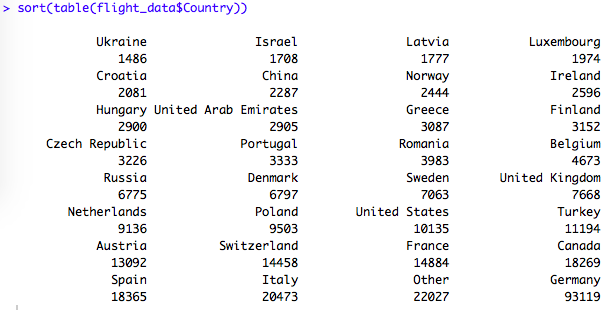
\includegraphics[width=\textwidth]{Figures/other_country.png}
    \caption{Departure flights mapped to countries}
    \label{fig:other_country}
\end{figure}


%\begin{table}[H]
%\centering
%\begin{tabular}{||c c||} 
%\hline
%Country & Frequency  \\ [0.5ex] 
%\hline\hline
%Ukraine  &  1486 \\
%Israel  &  1708 \\
%Latvia  &  1777 \\
%Luxembourg  &  1974 \\
%Croatia  &  2081 \\
%China  &  2287 \\
%5Norway  &  2444 \\
%Ireland  &  2596 \\
%Hungary  &  2900 \\
%United Arab Emirates  &  2905 \\
%Greece   & 3087 \\
%Finland  &  3152 \\
%Czech Republic  &  3226 \\
%Portugal  &  3333 \\
%Romania  &  3983 \\
%Belgium  &  4673 \\
%ussia  &  6775 \\
%Denmark  &  6797 \\
%Sweden  &  7063 \\
%United Kingdom  &  7668 \\
%Netherlands  &  9136 \\
%Poland  &  9503 \\
%United States &  10135 \\
%Turkey &  11194 \\
%Austria  & 13092 \\
%Switzerland  & 14458 \\
%rance &  14884 \\
%Canada &  18269 \\
%Spain &  18365 \\
%Italy &  20473 \\
%Other &  22027 \\
%Germany  & 93119\\
%\hline \hline
%\end{tabular}
%\caption{Departure flights mapped to countries}
%\label{table:other_country}
%\end{table}

Adding the variable to our dataset though didn't improve the prediction much but it did slightly increase the correct prediction of class 2 and 3 as can be seen in figure \ref{table:rf_with_country}

\begin{table}[H]
\centering
\begin{tabular}{l | a | b | a | b | a}
\hline
\rowcolor{LightCyan}
\mc{1}{Actual Delay class}  & \mc{1}{Class 0} & \mc{1}{Class 1} & \mc{1}{Class 2} & \mc{1}{Class 3} & \mc{1}{Grand Total} \\
\hline
Class 0 & 71290 & 365 & 14 & 8 & 71677 \\
Class 1 & 6976 & 1214 & 50 & 5 & 8245\\ 
Class 2 & 976 & 160 & 159 & 4 & 1299\\
Class 3 & 332 & 13 & 11 & 65 & 421\\ \hline
Grand Total & 79574 & 1752 & 234 & 82 & 81642
\end{tabular}
\caption{Confusion matrix of random forest with added country variable}
\label{table:rf_with_country}
\end{table}

\subsection{XGBoost}
XGBoost is an optimised distributed gradient boosting library designed to be highly efficient, flexible and portable. It implements machine learning algorithms under the Gradient Boosting framework. These optimisations result in making XGBoost highly scalable for a large amount of data, using far fewer resources than existing systems.\cite{Chen2016XGBoost:System}
Gradient boosting of regression trees produces competitive, highly robust, interpretable procedures for both regression and classification, especially appropriate for mining less than clean data. \cite{Hastie2001TheIllustrations} Using XGBoost meant that all factor variables were be converted to indicator columns and dataset saved as a matrix and passed on to the model. The multiclass classification algorithm of XGBoost provides a probability of each class instead of predicting the actual class. The prediction after 200 rounds was as follows.

\begin{table}[H]
\centering
\begin{tabular}{l | a | b | a | b | a}
\hline
\rowcolor{LightCyan}
\mc{1}{Actual Delay class}  & \mc{1}{Class 0} & \mc{1}{Class 1} & \mc{1}{Class 2} & \mc{1}{Class 3} & \mc{1}{Grand Total} \\
\hline
Class 0 & 71204 & 541 & 15 & 10 & 71677 \\
Class 1 & 7614 & 583 & 36 & 4 & 8245\\ 
Class 2 & 1116 & 127 & 49 & 4 & 1299\\
Class 3 & 316 & 20 & 10 & 13 & 421\\ \hline
Grand Total & 80250 & 1271 & 110 & 31 & 81642
\end{tabular}
\caption{XGBoost with 200 rounds and evaluation criteria mlogloss}
\label{table:xgboost}
\end{table}
The results obtained using XGBoost were also not ideal. Even with just 12-15\%  error, these predictions were not suitable for the project, as the models overwhelmingly predicted the delay class 0. A new strategy had to be formulated for fixing this class imbalance problem.

\section{Fixing class imbalance problems}
The prediction error up till now has been hovering at about 15\%. But the absolute error in this case is misleading. As the number of flights which were on time is much larger than the number of flights that got delayed, even classifying every flight as not delayed will give an error rate of about 15\% in our dataset. This is known as class imbalance problem and needs to be fixed. One way of fixing the issue is giving weights to different classes based on the frequency of the class. In simple terms, the class with the highest frequency is given the lowest weight whereas the class with the lowest frequency is given the highest weight. The class imbalance issue was tried to be fixed using both XGBoost and randomforest algorithms.

\subsection{XGBoost}
XGBoost natively supports fixing class imbalance problem. It has a variable called \textit{scale\_pos\_weight} that is used to give weight to classes. But this value does not accept a vector. Instead it is just a value that is used as a weight for the positive class (in this case, the flight delayed class). This variable, by design, just works with binary classification. Even when tried for multiclass classification, the trained model just predicts the test dataset in binary as seen in table \ref{table:xgboost_w} .
\begin{table}[H]
\centering
\begin{tabular}{l | a | b | a}
\hline
\rowcolor{LightCyan}
\mc{1}{Actual Delay class}  & \mc{1}{Class 0} & \mc{1}{Class 1} & \mc{1}{Grand Total} \\
\hline
Class 0 & 32866 & 10946 & 43812 \\
Class 1 & 3879 & 1217 & 5096\\ 
Class 2 & 602 & 186 &  788\\
Class 3 & 219 & 77 & 296\\ \hline
Grand Total & 37566 & 12426 & 49992
\end{tabular}
\caption{XGBoost just predicts 1 or 0 if using scale\_pos\_weight}
\label{table:xgboost_w}
\end{table}
The other way to improve class imbalance problem was to use the evaluation metric as AUC, or Area under ROC curve. In an ROC curve the true positive rate (flights correctly predicted as delayed) is plotted in function of the false positive rate(flights incorrectly predicted as delayed). Instead of improving on basis of reducing absolute error, XGBoost instead tries to maximise area under ROC curve. But unfortunately, for multiclass classification, XGBoost doesn't allow AUC as an evaluation metric, only for binary classification. Consequently the idea of fixing class imbalance problem using XGBoost was dropped.


\subsection{Using Random Forest}
Similar to most classifiers, Random Forest can also suffer from the curse of learning from a highly imbalanced training data set. As it is constructed to minimise the overall error rate, it will tend to focus more on the prediction accuracy of the majority class, which often results in poor accuracy for the minority class.\cite{Chen2004UsingDatab}. In Random forest, the weight signifies the probability an observation is selected for the tree. Observations with higher weights are selected more frequently. The same package for Random Forest, \textit{ranger} will now be used with weights. This package expects a vector with the same length of the number of observations in the dataset. The weights were calculated on the basis of the frequency of classes. The weighted model didn't give any tangible improvements when the weight was calculated on the basis of inverse of frequency of classes. It was decided the ratio of weights should be even more amplified. A multitude of different weights were calculated but the one that gave the best result was this. 
    
\begin{lstlisting}[language=R, breaklines=true]
weights <- NULL
weights <- ifelse(train\$flight_delay_bins == "0", (1/table(train\$flight_delay_bins)[1]) * 0.10, 0)
weights <- ifelse(train\$flight_delay_bins == "1", (1/table(train\$flight_delay_bins)[2]) * 0.20, weights)
weights <- ifelse(train\$flight_delay_bins == "2", (1/table(train\$flight_delay_bins)[3]) * 0.30 , weights)
weights <- ifelse(train\$flight_delay_bins == "3", (1/table(train\$flight_delay_bins)[4]) * 0.40, weights)
\end{lstlisting}

This weight variable, finalised as a result of many trial and error efforts, along with the number of trees increased to 200, resulted in a marked improvement over the test prediction dataset. The confusion matrix, table \ref{table:rf_100_w}, has all it's diagonal elements maximised compared to the other results. In class 3, even though more classes are predicted as class 1, it is considered acceptable as more flights are still classified as delayed rather than on-time. This is the ideal prediction desired for the project's requirement.


\begin{table}[H]
\centering
\begin{tabular}{l | a | b | a | b | a}
\hline
\rowcolor{LightCyan}
\mc{1}{Actual Delay class}  & \mc{1}{Class 0} & \mc{1}{Class 1} & \mc{1}{Class 2} & \mc{1}{Class 3} & \mc{1}{Grand Total} \\
\hline
Class 0 & 53710 & 17430 & 396 & 141 & 71677 \\
Class 1 & 2997 & 5054 & 168 & 26 & 8245\\ 
Class 2 & 348 & 706 & 235 & 10 & 1299\\
Class 3 & 123 & 185 & 30 & 83 & 421\\ \hline
Grand Total & 57178 & 23375 & 829 & 260 & 81642
\end{tabular}
\caption{Random forest with weighted variable}
\label{table:rf_100_w}
\end{table}

On just the accuracy basis, this algorithm is worse than before with about 25\% prediction error, much worse than 12-15\% achieved earlier. Nut based on the criteria for evaluating this prediction defined above, this was the best prediction.

\section{Prediction using regression}
Even though a good prediction was achieved using classification with weights, regression was also tested to see if it could preform better. In statistical modelling, regression is defined as the process to evaluate the degree of relationship among the data variables. For the platform, the target variable for regression model is arrival delay in seconds.

\subsection{Linear Modelling}
Beginning with the basics, the first algorithm chosen for regression was linear modelling using R function called \textit{lm}. Unfortunately the result of the model wasn't satisfactory. The adjusted R-squared value of the model was just .1272. A good result has an r squared value much closer to 1. As the result was so far from ideal, it was not considered for further improvements.

\subsection{Random Forest}
Random forest, already used as a classification algorithm, can also be utilised for a regression model. Using default parameters, and the target variable as arrival delay in minutes, the R-squared of the algorithm comes up to be .1319, as seen in figure \ref{fig:regression_rf_no_departure}. Again, this is not an ideal result. As both the results of the regression were terrible, the idea of prediction using regression was dropped.

\begin{figure}[H]
    \centering
    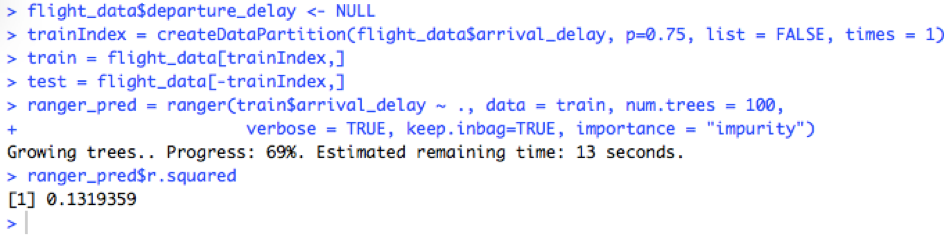
\includegraphics[width=\textwidth]{Figures/regression_rf_no_departure.png}
    \caption{Regression using Random Forest}
    \label{fig:regression_rf_no_departure}
\end{figure}

There is one thing to note that if the variable departure delay is used in the dataset, the predictions improve dramatically. The R-squared value for random forest improves from .13 to .86. Unfortunately it can't be used as this variable won't be available while predicting the flight delays for future flights.

\begin{figure}[H]
    \centering
    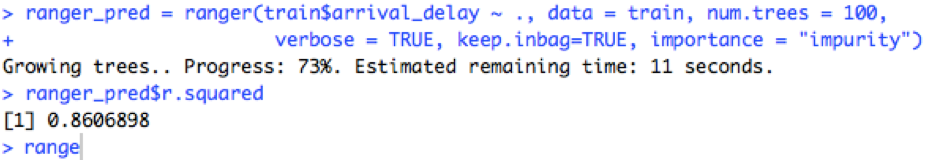
\includegraphics[width=\textwidth]{Figures/regression_rf.png}
    \caption{Regression using Random Forest, including departure delay}
    \label{fig:regression_rf}
\end{figure}


\section{Conclusion}
Based on the analysis done so far, the class imbalance problem was fixed to a large extent via using weights with random forest algorithm. Even though the absolute accuracy of the model decreases if using weights, this model is more suitable to the problem at hand and will be used as the algorithm for real-time flight delay prediction. % Prediction

\chapter{Website}

Now that we have discussed all the essential components required to create the website for users to purchase the insurance, we will move to discuss about the actual creation of the website. Our website will be based on a single most important principle: Simplicity. The user will never get to see any technical jargon or need to interact with useless webpages going through things that don't matter to them. Our aim is to make the whole process of buying insurance so simple that the user can but the insurance in three clicks and if the flight is delayed, gets his/her payout automatically. 
\\The insurance process will be carried out with a web app that has been up and running on a publicly accessible server, \url{insurance.pythonanywhere.com}. In this chapter we will first go through all the technologies used to create the website and then go through all the components of the website. 

\section{Technologies Used}
There are multiple technologies that go towards making a full fledged user-facing website. We will discuss all the technologies used and the reasons they were used. Apart from blockchain, we won't go deep into any other technology as it will be out of scope of this paper. 

\subsection{Python}
Python is a dynamically scripted language that has become immensely popular in recent times due to its simplicity and huge developer support. For our project, the following two were the criteria on the basis of which Python was selected as the programming language of choice:
\begin{enumerate}
    \item Web frameworks
    \\Python has very popular native web-frameworks such as Django and flask. Both have great documentation and developer support, essential for this project. 
    \item Data science libraries
    \\ Apart from R, python is the language with most support for the data science libraries and a go to choice for data science algorithms implementation. Even though as already mentioned in the previous chapter that our prediction algorithms were created in R, the final implementation of the algorithms has to be in our web framework language. Hence the availability of such algorithms' native implementation in python was a important consideration
\end{enumerate}

\subsection{Flask}
Flask is one of the most popular frameworks in Python. Even though Django is considered to be more mature platform with higher developer support, flask is easier to start with and had everything that was essential to create the website for us. 

\subsection{MySQL}
MySQL was chosen as a default choice as our database wasn't going to be a complex database. 

\subsection{PyCharm IDE}
PyCharm was the Python IDE of choice for the development process as it was a free choice with native support for flask framework. It also has inbuilt support for version control system.

\subsection{Github}
For software version management, Github was chosen for version control, being the most popular git client. The public account was chosen to create the repository, as it was free and the project does not require any privacy features at the moment.

\section{Website Structure}
The structure of the website consists of the separate aspects of the website at the backend that help in creating the website. 
\subsection{User Administration}
The starting point for every user, user administration is responsible for:
\begin{enumerate}
    \item Registering a user
    \item Logging in a user
    \item Maintaining a user session
\end{enumerate}
A Flask library called flask\_login was used to implement the User administration aspect of the website.

\subsection{SQL model}
The SQL model defines the database model that will be used by the website for keeping user records and flight/insurance details. It contains multiple classes that correspond to unique tables in MySQL database. The first class/model defines the table structure of all the important details for the website:
\begin{itemize}
    \item First name
    \item Last name
    \item Email Address
    \item Password
    \item Flight ID
    \item Date
    \item Insurance ID
    \item Blockchain status
    \item Blockchain receipt
    \item Multiple payout amounts for different categories of delays
\end{itemize}

The second class/model defined creates a MySQL table that is used for our autocomplete feature on the website. Our website will only deal with airlines that land in Germany, hence we have to limit the ability of user to enter a limited set of flights. This is done using the autocomplete feature of jQuery. This model contains all the flight details including origin, destination, airline etc. Once a user starts entering flight ID in the Flight ID field, the options are presented from our database using autocomplete function of jQuery. The user is not allowed to enter any other Flight ID. 

\subsection{Forms}
Forms are the flask's rendition of the HTML5 form fields. It creates HTML5 fields but adds input validation to them and makes them easier to use within our webapp. The library used for flask forms is called as WTforms. 

\subsection{Views}
Views are basic functions that explain the framework what to do for each URL. For ex. we have a login URL for which the login view will be called. Create insurance view will call a view function attached to it's URL and so on. What we generally do is import a form to a view function if any user input is required, perform any function if required on the fields and display it to the user.

\subsection{REST API calls}
REST API is a important component of any dynamic web application today. We use the Request module of Python to make a REST API call whenever we require some data from a third party, like weather, flight data or blockchain anchoring.

\subsection{Email Notifications}
The user has to be notified each time an insurance is created as well as when we have the flight status once the flight has landed. The notifications are currently being sent using my gmail address using a python library called \textit{smtplib}. The user details are taken from the user table, with the flight status, if available, from a REST API call. We add the details to a variable and send that variable to gmail's SMTP server with our own user account details.

\subsection{Blockchain}
As discussed in the blockchain chapter, we use Tierion API to hash our data and anchor it to the blockchain. This is done through a REST API call with user data sent as body in a HTTPS POST request. We receive the id of the request as the response which we store as Insurance ID. We use the same insurance ID to get the blockchain receipt once it's anchored to the blockchain.

\subsection{Insurance payout}
We create a script that runs once everyday with help of cron jobs. The aim of the website is to get the flight status of each flight for which we have created an insurance. If it finds out the status of a flight, based on that an email notification is created stating how much the flight was delayed and the corresponding payout. 

\section{Website Details}
No matter how good we handle things at the backend, the Frontend has to simple enough for the user to buy insurance easily. In this section we will go through all the sections of the website. 

\subsection{Registration Page}
This will be the initial page for each user for using the website. As can be seen in the \ref{fig:reg_page}, we just require basic details from the user to get the account ready. All the fields have complete string validation with Email field requiring the value entered to be in the Email format. On clicking register, the values are validated and saved in the database. The user is redirected to the login page.

\begin{figure}[h]
    \centering
    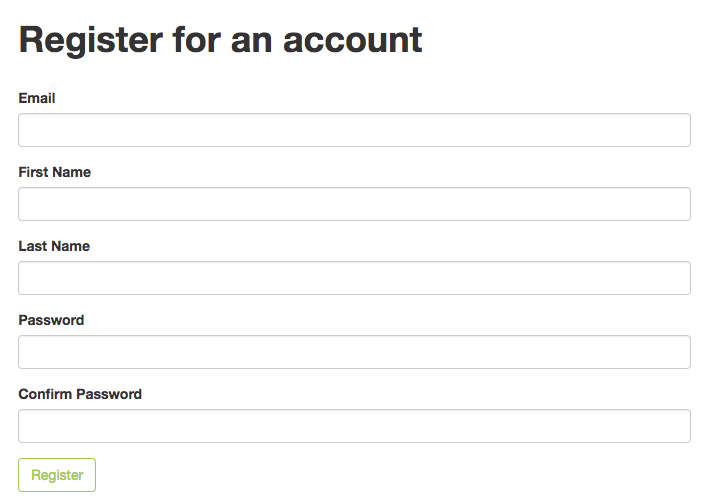
\includegraphics[width=\textwidth]{Figures/registration_page.png}
    \caption{Registration page}
    \label{fig:reg_page}
\end{figure}

\subsection{Login Page}
This is a simple login page. The user has to enter the Email ID and password and press Login. 
\begin{figure}[h]
    \centering
    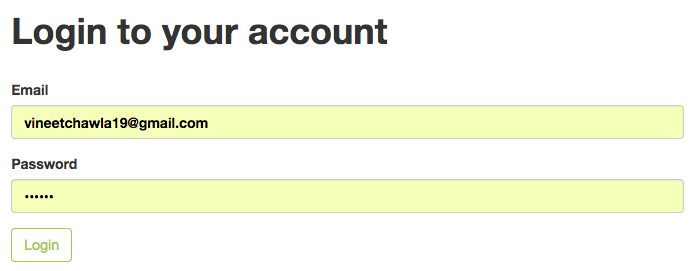
\includegraphics[width=\textwidth]{Figures/login_page.png}
    \caption{Login page}
    \label{fig:login_page}
\end{figure}

\subsection{Initial Dashboard}
The initial dashboard will be blank except for option for adding an insurance.
Once the user selects \textit{Add Insurance}, the user is redirected to Fight details webpage.
\begin{figure}[h]
    \centering
    
\includegraphics[width=\textwidth]{Figures/init_dashboard.png}
    \caption{Initial Dashboard}
    \label{fig:init_dash}
\end{figure}


\subsection{Header/Footer}
There are multiple values that are set dynamically in our header:
\begin{itemize}
    \item The rightmost field in the header is always \textit{Hi\,first\_name}.
    \item Once the user logs out, the Logout button is changed to login.
    \item The link to website's codebase in Github is also available in header.
\end{itemize}

\begin{figure}[h]
    \centering
    
\includegraphics[width=\textwidth]{Figures/header.png}
    \caption{Permanent Header. The rightmost field uses the user's first name.}
    \label{fig:header}
\end{figure}

\subsection{Flight Details}
The flight details page is the first part of the process of booking insurance for the user. Even though there are many fields visible to the user, only two fields can be filled by user input:
\begin{itemize}
    \item Flight ID
    \\This is a drop down list where as soon as the user enters two characters, the valid flight IDs will be automatically suggested.  On selecting a flight, automatically all the fields are populated with details of the flight selected. Only the suggest flight IDs will be considered valid for insurance. This auto completion is achieved using jQuery.
    \item Date
    \\ A simple date field for entering the date of the flight departure.
\end{itemize}
Once the user selects the Flight ID and date and presses \textit{Calcuate Insurance rates}, the user is redirected to the screen with insurance payout visibe.

\begin{figure}[h]
    \centering
    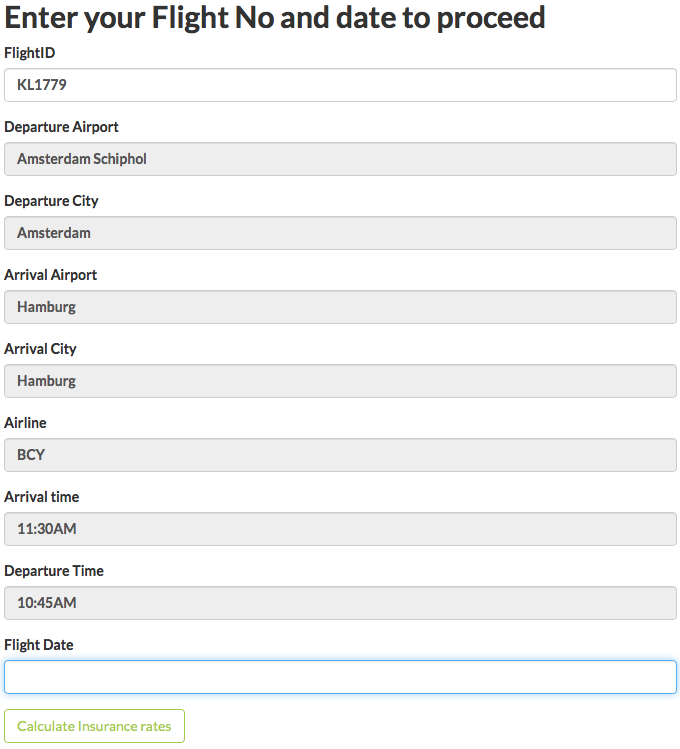
\includegraphics[width=\textwidth]{Figures/flight_details.png}
    \caption{Permanent Header. The rightmost field uses the user's first name.}
    \label{fig:flight_details}
\end{figure}

\subsection{Insurance Rates}
Even though we redirect from the previous page to this page, a whole lot of processing happens between the redirect page. We get all the flight details, we get the weather data for flight time at the selected date, fit the data in our model and predict the flight delay. Based on the flight delay, we calculate the insurance payout for each category of delay. Those rates are what displayed on this page. 
%%Add insurance screenshot
\\In a bid to be transparent, we present the user with payouts before they actually buy the insurance. If the user is satisfied with the rates he/she can move ahead and Buy insurance.

\subsection{Dashboard}
On buying the insurance, the user is redirected to the dashboard, but this time the user will have a new table on the dashboard. This table contains all the details of the insurance the user purchased along with the available blockchain anchoring proof, once available. Blockchain anchoring takes time due to fundamental design of how Bitcoin works. Hence the blockchain receipt is not initially available. That's why just after creating the insurance, your dashboard will have the blockchain status as unpublished as seen in figure \ref{fig:mid_dashboard}

\begin{figure}[h]
    \centering
    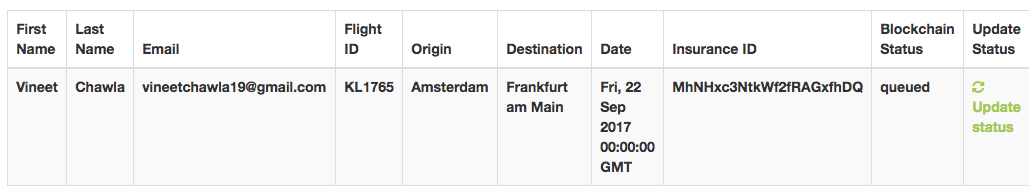
\includegraphics[width=\textwidth]{Figures/mid_dashboard.png}
    \caption{Insurance created but user details haven't been anchored to blockchain yet}
    \label{fig:mid_dashboard}
\end{figure}

The status update button is available on the dashboard, and pressing it refreshes the status. Within 10 minutes, we will have a blockchain status as complete and blockchain receipt in the box below the table as shown in figure \ref{fig:complete_dashboard}

\begin{figure}[h]
    \centering
    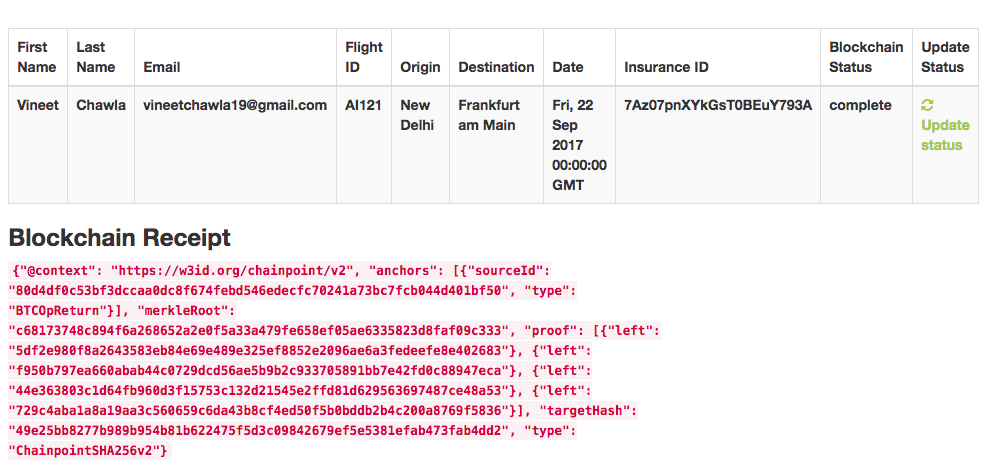
\includegraphics[width=\textwidth]{Figures/complete_dashboard.png}
    \caption{The Blockchain receipt is available and status has been updated}
    \label{fig:complete_dashboard}
\end{figure}

\subsection{Blockchain Receipt}
As shown in the last section, blockchain receipt is updated within ten minutes of creating the insurance. But what is blockchain receipt and what does it signify, we need to emphasise. Firstly the fields in blockchain receipt as show in table \ref{table:receipt}

\begin{table}[h!]
\centering
\begin{tabular}{||c c||} 
 \hline
 Name & Description  \\ [0.5ex] 
 \hline\hline
@context & the JSON-LD context for the receipt \\ 
\hline
type & receipt type definition specifying hash method and version \\
\hline
targetHash & hash value being anchored to the blockchain \\
\hline
merkleRoot	& merkle tree root value that is anchored to the blockchain \\
\hline
proof	& merkle proof establishing link from the targetHash to the merkleRoot \\
\hline
anchor-type	& anchor type definition specifying anchoring method (always bitcoin in our case \\
\hline
anchor-sourceId &	identifier, such as a transaction id, used to locate anchored data \\ [1ex]
 \hline
\end{tabular}
\caption{Different fields in blockchain receipt}
\label{table:receipt}
\end{table}

%%Explain significance of blockchain receipt


\section{Cloud Provider}
For cloud provider, the consideration was a web hosting company rather than cloud service providers like Amazon and Google. Hence we went with pythonanywhere.com. Instead of providing with empty VM's, it tries to automate most of the tedious work of setting up the web server. Even the database creation and initialisation is automated. 
The setup ensured that we don't have to manage our own web server or maintain a linux machine. Once we uploaded our code from github and initialised MySQL, the website was ready to go.
The tier chosen is just 5€ per website and scales dynamically, providing us with external internet connections too.

\section{Security Features}
Even though this is not a security project, the website security has been given utmost importance.
\begin{enumerate}
    \item HTTPS
    \\ We use a HTTPS certificate from Lets Encrypt to encrypt our connection.This maintains the privacy of connection and makes sure our connection doesn't leak any confidential data.
    \item Passwords are always stored as hashes. So in case of an attack, the attacker will never get to know the real passwords.
    \item There is not a single SQL query in the entire application. Creating SQL queries is handled by the API SQLAlchemy instead, we just pass parameters to the desired functions. Hence completely removing the possibility of SQL injection attacks
    \item Every user input is validated at the client side as well as server side
    \item Session variables are encrypted to prevent data leakage if website is accessed using public networks
\end{enumerate}

 % Website

\chapter{Conclusion} % Results and Discussion

%% ----------------------------------------------------------------
% Now begin the Appendices, including them as separate files

\addtocontents{toc}{\vspace{2em}} % Add a gap in the Contents, for aesthetics

\appendix % Cue to tell LaTeX that the following 'chapters' are Appendices


	% Appendix Title

%\input{Appendices/AppendixB} % Appendix Title

%\input{Appendices/AppendixC} % Appendix Title

\addtocontents{toc}{\vspace{2em}}  % Add a gap in the Contents, for aesthetics
\backmatter

%% ----------------------------------------------------------------
\label{Bibliography}
\lhead{\emph{Bibliography}}  % Change the left side page header to "Bibliography"
\bibliographystyle{unsrtnat}  % Use the "unsrtnat" BibTeX style for formatting the Bibliography
\bibliography{mendeley}  % The references (bibliography) information are stored in the file named "Bibliography.bib"

\end{document}  % The End
%% ----------------------------------------------------------------